Die Messapparatur ist zusammengesetzt aus einen Rechner, einem Ultraschallgerät und einem Schallkopf ($f=\SI{2}{MHz}$).
Auf dem Ultraschallgerät lassen sich auch Verstärker einstellen, die in beliebiger Tiefe das Signal verstärken.
Zunächst wird ein Acrylblock mit verschiedenen Störstellen (Abb. \ref{fig:block}) mit A-Scans und B-Scans untersucht.
\begin{figure}[h!]
  \centering
  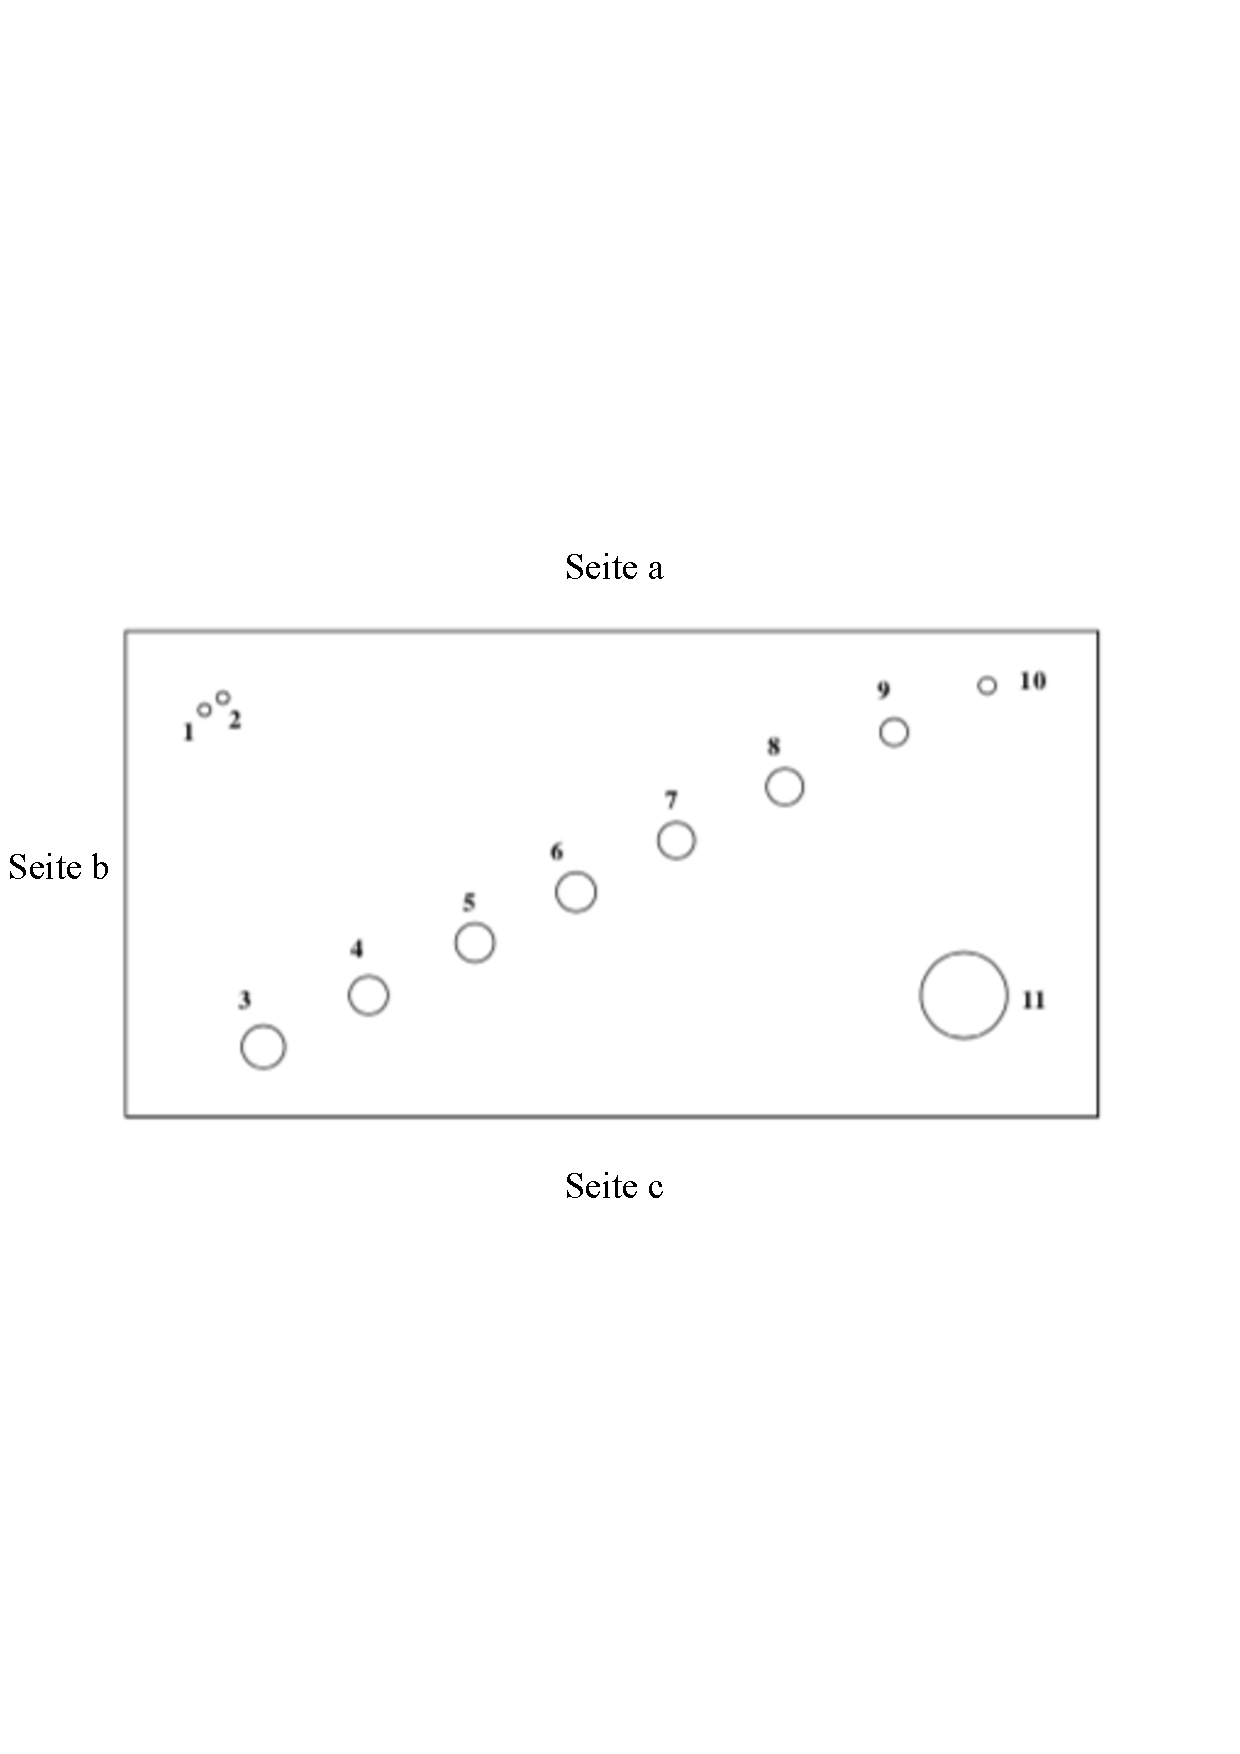
\includegraphics[width=\textwidth]{block.pdf}
  \caption{Untersuchtes Objekt: Acrylblock mit Störstellen \cite{1}}
  \label{fig:block}
\end{figure}
Als erstes werden der Acrylblock und die Störstellen mit einer Schieblehre vermessen.
Im Rechner wird die Schallgeschwindigkeit in Acryl eingegeben: $c_{\text{Acryl}}=\SI{2730}{\frac{m}{s}}$ \cite{acryl}
Dazu wird als Kontaktmittel destilliertes Wasser verwendet.
\\Der Acrylblock wird von Seite a mit einem A-Scan durchschallt.
Der gemessene Abstand der Störstelle zum Schallkopf wird notiert.
Die Messung wird für die Störstellen 3-9 durchgeführt.
Anschließend wird die Messung an Seite c wiederholt.
\\Die Störstellen 1 und 2 werden von den Seiten a, b und c vermessen, um den Abstand zwischen ihnen errechnen zu können.
\\Der Acrylblock wird nun mithilfe von B-Scans untersucht.
Dazu wird wieder destilliertes Wasser als Kontaktmittel verwendet.
Der Schallkopf wird erst langsam über die Seite a bewegt.
Auf dem Bildschirm erscheint ein zweidimensionales Bild.
Die Abstände der Störstellen zum Schallkopf werden dem Bild entnommen.
Analog wird die Messung von Seite c aus durchgeführt.
\\Für die TM-Scans wird ein anderes Objekt geschallt.
Ein Modell eines Herzens, bestehend aus einer Handpumpe, einem Plasikgefäß mit einer elastischen Membran, auf der ein Wasserspiegel steht.
Der Schallkopf wird so arritiert, dass er grade eben die Wasseroberfläche berührt.
Als Schallgeschwindigkeit in Wasser wird $c_{\text{Wasser}}=\SI{1485}{\frac{m}{s}}$ \cite{acryl} eingestellt.
Mit der Handpumpe wird gleichmäßig gepumpt, so dass sich die Membran und entsprechend der Wasserspiegel heben und senken.
Auf dem Rechner erscheint ein Bild, auf dem die Pumpvorgänge deutlich erkennbar sind.
Aus der Amplitude der 'Herzschläge' wird das Schlagvolumen bestimmt.
Vom Bildschirm kann die Herzfrequenz abgelesen werden.
